% =====================================================================
%  第 6 章 §6.2 后半（原书 p.261–275 / PDF 271–285）—— ch06a2
%  续写；不写章标题与节标题
% =====================================================================

% [原文 p.261]
论，与 $CM_{g,k}$ 的情形相同，适当的稳定性定义是要点之一。

\begin{definition}{6.42}
  设 $\Sigma$ 为半稳定曲线。连续映射 $\varphi:\Sigma\to M$ 是\textbf{伪全纯的}（pseudoholomorphic），是指 $\varphi$ 诱导到正规化 $\bigcup\Sigma_i$ 的映射 $\bar\varphi:\bigcup\Sigma_i\to M$ 是伪全纯的。

  设 $\varphi:\Sigma\to M$、$\varphi':\Sigma'\to M$ 为伪全纯映射。使 $\varphi'\circ\psi=\varphi$ 的正则同构 $\psi:(\Sigma,\vec z)\to(\Sigma',\vec z')$ 称为 $(\Sigma,\vec z,\varphi)$ 与 $(\Sigma',\vec z',\varphi')$ 之间的\textbf{同型}。$(\Sigma,\vec z,\varphi)$ 与自身的同型全体构成群，记作 $\mathrm{Aut}(\Sigma,\vec z,\varphi)$。

  $(\Sigma,\vec z,\varphi)$ 称为\textbf{稳定映射}（stable map），是指 $\mathrm{Aut}(\Sigma,\vec z,\varphi)$ 为有限群。
\end{definition}

若 $(\Sigma,\vec z)$ 稳定，则 $(\Sigma,\vec z,\varphi)$ 也稳定，但逆一般不成。

\begin{lemma*}{6.43}
  $(\Sigma,\vec z,\varphi)$ 稳定，等价于对任意非奇异不可约成分 $\Sigma_i$，下列条件 (1)、(2) 之一成立：
  \begin{enumerate}[label=（\arabic*）]
    \item 设 $\Sigma_i$ 的亏格为 $g_i$、特殊点数为 $k_i$，则 $2g_i+k_i\ge3$；
    \item $\varphi$ 在 $\Sigma_i$ 上诱导的映射不是常值映射。
  \end{enumerate}
\end{lemma*}
\begin{proof}
  设存在不满足 (1)、(2) 的非奇异不可约成分 $\Sigma_i$。则 $\Sigma_i$ 的、不动特殊点的自同构有无穷多个。将其在 $\Sigma_i$ 之外延拓为恒等映射，得到 $(\Sigma,\vec z)$ 的自同构 $\psi$。在 $\Sigma_i$ 的像上 $\varphi$ 是常值映射，故 $\psi$ 是 $(\Sigma,\vec z,\varphi)$ 的自同构。即 $\mathrm{Aut}(\Sigma,\vec z,\varphi)$ 是无限群。

  证明逆。不可约成分只有有限个，故 $\mathrm{Aut}(\Sigma,\vec z,\varphi)$ 中不置换不可约成分者全体 $\mathrm{Aut}_0(\Sigma,\vec z,\varphi)$ 的指数有限。因此只需证 $\mathrm{Aut}_0(\Sigma,\vec z,\varphi)$ 有限。$\mathrm{Aut}_0(\Sigma,\vec z,\varphi)$ 是非奇异不可约成分 $\Sigma_i$ 的、固定特殊点并保持 $\varphi$ 的自同构全体 $\mathrm{Aut}(\Sigma_i)$ 的直积 $\prod\mathrm{Aut}(\Sigma_i)$。逐个不可约成分考虑。若 (1) 成立，非奇异不可约成分 $\Sigma_i$ 的、保持特殊点的自同构只有有限个。

  设 (2) 成立。若非奇异不可约成分的、保持 $\varphi$ 的自同构有无穷多个，
% [原文 p.262]
  则它们构成正维数的李群 $G$\footnote{证明略。这是复分析的一个好习题。}。$\varphi_i$ 拉回到 $\Sigma_i$ 后在每点的微分，在 $G$ 的轨道方向上为 $0$。由伪全纯性，若微分在某个方向为 $0$，则在其他方向也为 $0$。因此 $\varphi_i$ 到 $\Sigma_i$ 的拉回成为常数，矛盾。
\end{proof}

稳定映射 $(\Sigma,\vec z,\varphi)$ 的同调类由 $\sum_i\varphi_{i*}[\Sigma_i]\in H_2(M;\Z)$ 定义。这里 $\varphi_i$ 是 $\varphi$ 在 $\Sigma_i$ 上诱导的伪全纯映射。

\begin{definition}{6.44}
  同调类为 $\beta$ 的亏格 $g$ 的 $k$ 点稳定映射全体，记作 $CM_{g,k}(M,J_M;\beta)$。
\end{definition}

\begin{theorem}{6.45}
  $CM_{g,k}(M,J_M;\beta)$ 是紧致且 Hausdorff 的。
\end{theorem}

\begin{remark}{6.46}
  严格地说，不先确定拓扑，定理 6.45 就没有意义。
\end{remark}

定理 6.45 证明的本质部分，是用 Sacks–Uhlenbeck 的想法所作的 Gromov 讨论，已在第 2 章说明。与 Gromov 的许多其他论文一样，[159] 中证明细节的省略也很多\footnote{但事后看来，要点其实全都写出来了。这与 Gromov 的许多其他论文一样。}。关于紧致性，这一点由 Pansu 的解说 [298] 补足。后来出现了 [299], [404] 等文献，[184], [253] 等也有解说。

\begin{remark}{6.47}
  关于 Hausdorff 性，长期以来是含糊的。稳定曲线这一概念是 Kontsevich 的（[218], [222]）。Gromov 使用了“尖点曲线”（cusp curve）一词。尖点曲线与稳定曲线是否指同一个东西，笔者至今不清楚。尖点曲线这一术语，事到如今还是不用为妥。

  如已说明，稳定性与 Hausdorff 性深刻相关。Pansu [298] 明言，依拓扑取法的不同，所得的紧化可能不是 Hausdorff 空间。这一点在其他文献中更含糊，甚至有不加说明就使用非 Hausdorff 拓扑的情形。明确指出稳定曲线模空间是 Hausdorff 空间的，大概首推 Kontsevich 的论文 [218]。写出 Hausdorff 性严格证明的文献，是 Fukaya–Ono [124] §10、§11 与 Siebert [333]。
\end{remark}

% [原文 p.263]

在 Calabi–Yau 流形情形，$CM_{g,k}(M,J_M;\beta)$ 对所有的 $\beta$ 都成为正确维数、即 $2(c^1(\beta)+n+3g-3+k)$ 维的光滑流形，其实绝不可能。但精确叙述这一点会使话题复杂，所以暂且闭眼承认 6.28 而先往前走。

一旦承认 6.28，Gromov–Witten 不变量的定义就已在前面说明过了。下面说明当时保留的定理的证明。

首先谈定理 6.30。定理 6.30 证明的想法已在第 2 章说明。即，有两个近复结构 $J_1$ 与 $J_2$ 时，取连接它们的近复结构之路 $J_\tau$，让 $\tau$ 变动，考虑关于 $J_\tau$ 的稳定曲线模空间之和 $\bigcup_\tau CM_{g,k}(M,J_\tau;\beta)$，就得到 $CM_{g,k}(M,J_1;\beta)$ 与 $CM_{g,k}(M,J_2;\beta)$ 之间的配边。由此定理 6.30 可得。
% [Tutor Note: 这里的关键是“配边”而非“同构”：$J_\tau$ 的取法可以不同，但 $\bigcup_\tau$ 的边界是两端模空间的不交并，故两端的 GW 不变量作为配边不变量相等。这正是第 2 章“用近复结构之路比较不变量”的手法。]

\begin{remark}{6.48}
  即使不固定辛结构而连续变动，$GW_{g,k}(M,J_M;\beta)$ 也不变。证明也与定理 6.30 相同。
\end{remark}

其次叙述引理 6.18 的证明。使用加强定理 6.45 的下述引理。

\begin{lemma}{6.49}
  对任意 $E$，并集
  \[
    \bigcup_{\beta\cap\omega_M\le E}CM_{g,k}(M,J_1;\beta)
  \]
  是紧的。
\end{lemma}

如第 2 章所述，伪全纯曲线列存在收敛子列的重要条件是能量的有界性。因此，定理 6.45 的紧致性证明，实际上是在证明引理 6.49。

由引理 6.49，满足 $CM_{g,m}(M,J_1;\beta)\neq\emptyset$ 且 $\beta\cap\omega_M<E$ 的 $\beta$ 只有有限个。因此存在列 $\beta_0=0,\beta_1,\dots$，满足下述条件 6.50。

\textbf{条件 6.50}
\begin{enumerate}[label=（\arabic*）]
  \item $\omega_M\cap\beta_i\le\omega_M\cap\beta_{i+1}$；
  \item $\lim_{i\to\infty}\omega_M\cap\beta_i=\infty$；
  \item 若 $CM_{g,m}(M,J_1;\beta)\neq\emptyset$，则存在 $i$ 使 $\beta=\beta_i$。
\end{enumerate}
% [Tutor Note: 引理 6.49 只保证能量有界的 $\beta$ 有限，故可按 $\omega_M\cap\beta$ 递增排列成 $\beta_i$；第三条是说凡出现过的同调类都在这个列表里。原书这里把点标数写成 $m$，与定义 6.44 的 $k$ 不一致，读时按 $k$ 理解。]

% [原文 p.264]
因此可写作
\[
  \mathrm{m}_2^A(P,Q)=\sum_i\mathrm{m}_2^{A,\beta_i}(P,Q)T^{\omega_M\cap\beta_i}\otimes u^{c^1(M)\cap\beta_i}.
\]
右边属于 $H^*(M;\Lambda_{nov})$ 这一点，由 Novikov 环的定义与条件 6.50 的 (2) 显然。（计算次数可知，除 $-2n\le c^1(M)\cap\beta_i\le2n$ 的 $\beta_i$ 以外 $\mathrm{m}_2^{A,\beta_i}$ 都为 $0$，因此在 $u$ 的指数上只出现有界范围内的整数。）这样引理 6.18 就证明了。

转到定理 6.19 的证明。首先证明式 (6.3)。对几何链 $(P_1,\psi_1)$、$(P_2,\psi_2)$、$(P_3,\psi_3)$，
\begin{align}
  &\langle \mathrm{m}_2((P_1,\psi_1),(P_2,\psi_2)),(P_3,\psi_3)\rangle_A \notag\\
  &\quad=\sum_\beta\#\left((P_1\times P_2\times P_3)_{\psi_1,\psi_2,\psi_3}\times_{ev}CM_{0,3}(M,J_1;\beta)\right)\otimes T^{\omega_M\cap\beta}\otimes u^{c^1(M)\cap\beta} \tag{6.11}
\end{align}
（$\#$ 表示计入符号后的个数）。求和取遍满足 $\mathrm{codim}\,P_1+\mathrm{codim}\,P_2+\mathrm{codim}\,P_3=\dim CM_{0,3}(M,J_1;\beta)$ 的 $\beta$ 全体。由于 (6.11) 除符号外在 $P_1,P_2,P_3$ 的循环置换下不变，故式 (6.3) 得证。（符号的讨论在本书中一概省略。）
% [Tutor Note: $\#$ 是模空间的“虚拟”计数，即按定向计入符号的交点数；作者在全书一律省略符号的讨论，故此处只需按有符号计数理解，具体符号约定见 [124]。]

结合律由下述定理得出。

\begin{theorem}{6.51}
  \[
    \sum_{\beta_1+\beta_2=\beta}\mathrm{m}_{2,\beta_1}^A\left(\mathrm{m}_{2,\beta_2}^A(P_1,P_2),P_3\right)=\sum_{\beta_1+\beta_2=\beta}\mathrm{m}_{2,\beta_1}^A\left(P_1,\mathrm{m}_{2,\beta_2}^A(P_2,P_3)\right).
  \]
\end{theorem}

\begin{remark}{6.52}
  结合律相当于弦理论中的\textbf{交叉对称性}（exchange symmetry）（见注 6.54）。交叉对称性从弦理论发端时起就为人所知，是提出弦理论的动机之一（见 [155] 的 Chapter 1）。明确叙述拓扑弦理论或 A 模型情形、即此处所论情形的结合律的，是 Vafa [373] 最早。

  在数学论文中证明结合律的，是在半正情形下证明的 Ruan–Tian [319] 与 McDuff–Salamon [253] 最早。Kontsevich–Manin [222] 把包括结合律在内的 Gromov–Witten 不变量应满足的性质，整理成公理的形式，
% [原文 p.265]
  一般情形下 Gromov–Witten 不变量的定义与 Kontsevich–Manin 公理的证明，在射影代数簇情形由 [234], [39], [40] 给出，在辛流形情形由 [124], [235], [333], [317] 给出。
\end{remark}

Gromov–Witten 不变量的发现可以追溯到更早。Gromov–Witten 不变量定义的思路，即考虑伪全纯曲线模空间的基本同调类这一想法，已经出现在 Gromov 的论文 [159] 中，McDuff 等人随后的论文 [251], [252] 也有效地使用了它。Ruan 在 [315], [316] 中把这一想法显在化，明确定义了不变量并给出其应用。

另一方面，用近复结构作\textbf{拓扑 $\sigma$ 模型}（topological sigma model），是 Witten 的论文 [392] 所做的。更准确地说，Witten 对近复流形，在能量（定义 2.69）上添加费米子部分使之超对称，再加上\textbf{拓扑扭转}（topological twist），考虑了这样得到的拉格朗日泛函。考虑其费曼路径积分（Feynman path integral），由于有拓扑扭转，超对称性导致相消，费曼路径积分的值在近复结构等形变下不变。（这一讨论是椭圆型算子指数的拓扑不变性的物理学式“证明”的非线性化。）这样得到的不变量与 Gromov–Witten 不变量一致。

以上讨论是形式讨论。要使伪全纯结构在连续形变下的不变性成立，近复结构必须对某个辛结构 $\omega$ 是 $\omega$-\textbf{温和}（tame）的\footnote{关于这一点，§2.5 有详细说明。}。这一点在 [392] 中似乎未被认识到。基于超对称性与路径积分的物理学式讨论能否说明辛结构的必要性，笔者不知道。
% [Tutor Note: “$\omega$-温和”即通常所说的 $\omega$-tame：$\omega(v,Jv)>0$ 对一切非零切向量成立。它是模空间紧致性（第 2 章）所需的全部假设；若去掉它，伪全纯曲线可能退化到无穷，GW 不变量就不一定有定义。]

\begin{proof}[定理 6.51 的证明]
  这里承认 6.28 来证明。设 $(P_1,\psi_1)$、$(P_2,\psi_2)$、$(P_3,\psi_3)$ 为 $M$ 的几何链。把纤维积
  \[
    (P_1\times P_2\times P_3)_{\psi_1,\psi_2,\psi_3}\times_{ev_1,ev_2,ev_3}CM_{0,4}(M,J_M;\beta)
  \]
  记作 $\mathcal X$。考虑代入映射 $ev_4:\mathcal X\to M$ 与忘却映射 $\mathrm{fg}:\mathcal X\to CM_{0,4}$。如例 6.40 所述，$CM_{0,4}\cong\CP^1$，其中 3 点是 $CM_{0,4}-M_{0,4}$ 的点，即对应奇异的半稳定曲线。把图 6.5 的 (a)、(b) 对应的 $CM_{0,4}$ 的点分别记为 $a,b$。
\end{proof}

% [原文 p.266]
\begin{lemma*}{6.53}
  $(\mathrm{fg}^{-1}(a),ev_4)$ 是表示定理 6.51 左边的几何链，$(\mathrm{fg}^{-1}(b),ev_4)$ 是表示定理 6.51 右边的几何链。
\end{lemma*}
\begin{proof}
  只证前半。半稳定曲线记作 $(\Sigma,\vec z)$。$\mathrm{fg}^{-1}(a)$ 与使 $\varphi:\Sigma\to M$ 为伪全纯映射、且其同调类为 $\beta$ 者全体一致。$\Sigma=\Sigma_1\cup\Sigma_2$（含 $z_1,z_2$ 的一方为 $\Sigma_1$）。$\varphi$ 的同调类是 $\varphi_*[\Sigma_1]$ 与 $\varphi_*[\Sigma_2]$ 之和。把对应 $\varphi_*[\Sigma_1]=\beta_1$、$\varphi_*[\Sigma_2]=\beta_2$ 的 $\varphi$ 的部分记作 $\mathcal X(\beta_1,\beta_2)$。几何链
  \[
    \left((P_1\times P_2)_{\psi_1,\psi_2}\times_{ev_1,ev_2}CM_{0,3}(M,J_M;\beta_1),ev_3\right)
  \]
  按定义就是 $\mathrm{m}_{2,\beta_1}^A(P_1,P_2)$。把它记作 $(Q,ev_3)$，则
  \begin{align}
    &(Q\times P_3)_{ev_3,\psi_3}\times_{ev_1,ev_2}CM_{0,3}(M,J_M;\beta_2) \notag\\
    &\quad=(P_1\times P_2\times P_3)_{\psi_1,\psi_2,\psi_3}\times_{ev_1,ev_2,ev_3}\mathcal X(\beta_1,\beta_2) \tag{6.12}
  \end{align}
  (6.12) 的左边是 $\mathrm{m}_{2,\beta_2}^A(\mathrm{m}_{2,\beta_1}^A(P_1,P_2),P_3)$。由此得引理 6.53。
\end{proof}

\begin{proof}[定理 6.51 的证明（续）]
  完成定理 6.51 的证明。考虑连接 $a$ 与 $b$ 的道路 $\gamma:[0,1]\to CM_{0,4}$。用纤维积 $\mathcal Y=[0,1]\times_{\mathrm{fg}}CM_{0,4}(M,J_M;\beta)$，得到几何链
  \[
    \left((P_1\times P_2\times P_3)_{\psi_1,\psi_2,\psi_3}\times_{ev_1,ev_2,ev_3}\mathcal Y,ev_4\right).
  \]
  其边界是 $(\mathrm{fg}^{-1}(b),ev_4)-(\mathrm{fg}^{-1}(a),ev_4)$。因此由引理 6.53，定理 6.51 的右边与左边表示同一个同调类。
\end{proof}

\begin{remark}{6.54}
  图 6.5 的 (a)、(b) 的半稳定曲线对应的图 $\Gamma_\Sigma$，分别由图 6.7 给出。图 6.7 的两个费曼图（Feynman diagram）对应的微扰展开项的值一致，这就是交叉对称性。定理 6.51 证明中的讨论，可以说是它的拓扑类似物。
\end{remark}

\begin{figure}[htbp]
  \centering
  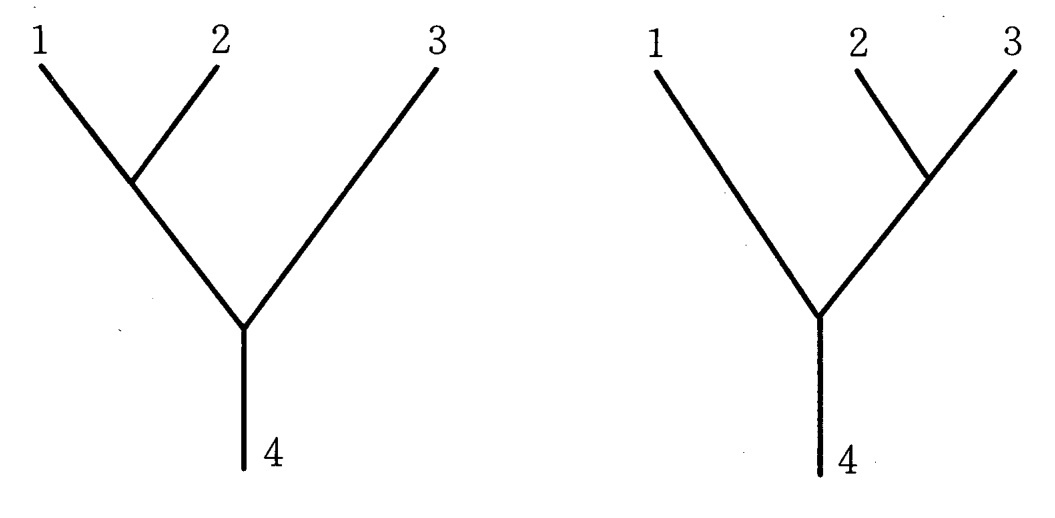
\includegraphics[width=0.62\textwidth]{figures/fig6.7.png}
  \figtitle{6.7}{交叉对称性（原书 p.267）}
\end{figure}

以上从 Gromov–Witten 不变量得到了以 Novikov 环为系数的上同调环的形变。称为\textbf{量子上同调环}（quantum cohomology ring）。

\begin{example}{6.55}
  设 $M=\CP^n$。设 $\CP^{n-1}$ 的基本同调类的 Poincaré 对偶为 $x$，则 $H^*(\CP^n;\Z)\cong\Z[x]/(x^{n+1})$。辛形式
% [原文 p.267]
  的上同调类是 $x$。$H_2(\CP^n;\Z)=\Z$，生成元是 $\CP^1$。令
  \[
    T^{\omega\cap[\CP^1]}\otimes u^{c^1(\CP^n)\cap[\CP^1]}=T\otimes u^{n+1}=q\in\Lambda_{nov}.
  \]
  由于 $\CP^n$ 是强正的，Gromov–Witten 不变量是整数系数同调类。又看定义可知，量子上同调环的系数可以是普遍 Novikov 环的子环 $\Z[q]$。（强正情形下，由次数计算可知 (6.6) 是有限和。）
  \begin{equation}
    \mathrm{m}_2^A(x^a,x^b)=
    \begin{cases}
      x^{a+b}, & a+b<n+1 \text{ 时},\\
      x^{a+b-n-1}\otimes q, & a+b\ge n+1 \text{ 时}
    \end{cases} \tag{6.13}
  \end{equation}
\end{example}

证明 (6.13)。$x^a$ 的 Poincaré 对偶是 $\CP^{n-a}$。$a+b<n+1$ 时，$\CP^{n-a}$ 与 $\CP^{n-b}$ 可经线性等价移动成横截，交是 $\CP^{n-a-b}$（当然这只是杯积的计算）。其他项由次数计算为 $0$。这就证明了 (6.13) 的第一式。
% [Tutor Note: $q$ 的次数是 $2(n+1)$，正好补上 $x^{a+b}$ 超出 $\dim_\C\CP^n=n$ 的部分；这就是量子上同调环中“$x^{n+1}=q$”这一关系的来源。]

$a+b\ge n+1$ 时，把 $\CP^{n-a}$ 与 $\CP^{n-b}$ 取成横截，则二者不相交。与 $\CP^{n-a}$ 和 $\CP^{n-b}$ 双方都相交的 1 次曲线（$\CP^1$）全体的并集，是 $\CP^{2n+1-a-b}$。实际上它对应于 $\CP^{n-a}$ 对应的 $\C^{n+1}$ 的部分向量空间（$n-a+1$ 维）与 $\CP^{n-b}$ 对应的 $\C^{n+1}$ 的部分向量空间的和空间，即 $\CP^{2n+1-a-b}$。由此得 (6.13) 的第二式。

量子上同调环的其他计算例见 [64] 等。迄今所做的计算与其说依据辛几何，不如说依据代数几何的手法，故这里不叙述。

% [原文 p.268]
Gromov–Witten 不变量比量子上同调环含有更多信息。例如，若 $y\in H_m(CM_{g,k+1})$，则用 $\mathrm{fg}^{-1}(y)\in H_m(CM_{g,k+1}(M,J_M;\beta))$ 的对应
\begin{equation}
  (P_1,\dots,P_k)\mapsto\left((P_1\times\dots\times P_k)\times_{ev_1,\dots,ev_k}\mathrm{fg}^{-1}(y),ev_k\right)T^{\beta\cap\omega_M}\otimes u^{c^1(M)\cap\beta} \tag{6.14}
\end{equation}
得到 $H(M;\Lambda_{nov})^{\otimes k}\to H(M;\Lambda_{nov})$ 的次数 $-m$ 的映射。

如注 6.52 所述，Gromov–Witten 不变量应满足的性质的公理化，由 Kontsevich–Manin [222] 完成。这里不逐条检查公理（见 [124] §23）。

要研究 Gromov–Witten 不变量跨所有亏格的结构，必须决定曲面模空间同调 $H_*(CM_{g,k};\Q)$ 的结构。$H_*(CM_{g,k};\Q)$ 的研究在许多人的努力下已有进展，但仍是困难之处很多的深刻问题。（[264] 有详细解说。）

这里就 $g=0$ 的情形再稍作叙述。特别是说明 §6.3、§6.4 中重要的 Comm$_\infty$ 代数的关系式（定理 6.59）\footnote{以下叙述参考了 Manin 的讲义 [242]。}。

在 (6.14) 中考虑 $y$ 为基本同调类 $[CM_{0,k+1}]\in H_{2k-4}(CM_{0,k+1};\Z)$ 的情形。即对几何链 $(P_i,\psi_i)$：

\begin{definition}{6.56}
  $\mathrm{m}_{k,\beta}^A$ 由下式定义：
  \[
    \mathrm{m}_{k,\beta}^A(P_1,\dots,P_k)=\left((P_1\times\dots\times P_k)\times_{ev_1,\dots,ev_k}CM_{0,k+1}(M,J_M;\beta),ev_{k+1}\right).
  \]
  以后用几何链 $(P,\psi)$ 作纤维积时，不再写出 $\psi$。
\end{definition}

定义 6.56 给出映射
\[
  \mathrm{m}_{k,\beta}^A:H^{m_1}(M;\Q)\otimes\dots\otimes H^{m_k}(M;\Q)\longrightarrow H^{m_1+\dots+m_k-2(c^1(M)\cap\beta)-2k+4}(M;\Q)
\]
（这里已用 Poincaré 对偶把同调与上同调等同起来。）

% [原文 p.269]
\begin{remark}{6.57}
  $k\le2$ 时 $M_{0,k}=\emptyset$，故其同调类没有意义，但定义 6.56 有意义。$\beta=0$、$k\le2$ 时 $M_{0,k}(M,J_M;\beta)=\emptyset$，故 $k\le2$ 时 $\mathrm{m}_{k,0}=0$。
\end{remark}

把 $H(M;\Lambda_{nov})^{\otimes k}\to H(M;\Lambda_{nov})$ 的次数 $-2k+4$ 的映射 $\mathrm{m}_k^A$ 由下式定义。
\begin{equation}
  \mathrm{m}_k^{A,fm}(P_1,\dots,P_k)=\sum_\beta\mathrm{m}_{k,\beta}^{A,fm}(P_1,\dots,P_k)T^{\beta\cap\omega_M}\otimes u^{c^1(M)\cap\beta}. \tag{6.15}
\end{equation}

\begin{lemma}{6.58}
  设 $P_i$ 的次数为 $m_i$，则下式成立：
  \[
    \mathrm{m}_k^{A,fm}(P_1,\dots,P_k)=(-1)^{m_im_{i+1}}\mathrm{m}_k^{A,fm}(P_1,\dots,P_{i+1},P_i,\dots,P_k),
  \]
\[
  \resizebox{0.97\linewidth}{!}{$\displaystyle \langle\mathrm{m}_k^A(P_1,\dots,P_k),P_{k+1}\rangle_{A,formal}=(-1)^{m_{k+1}(m_1+\dots+m_k)}\langle\mathrm{m}_k^{A,fm}(P_{k+1},P_1,\dots,P_{k-1}),P_k\rangle_{A,formal}. $}
\]
\end{lemma}

证明与定理 6.19 的证明中定义 6.7 的 (5)、(7) 的证明同样，故省略。

结合律的推广是下一定理。令 $I=\{4,\dots,m\}$。当 $J\subset I$ 时，把 $J$ 的元素从小到大排列为 $j_1,\dots,j_{\#J}$。令 $P_J=(P_{j_1},\dots,P_{j_{\#J}})$。又当 $J_1\cap J_2=\emptyset$、$J_1\cup J_2=I$ 时，写作 $J_1+J_2=I$。

\begin{theorem*}{6.59}
\[
  \resizebox{0.97\linewidth}{!}{$\displaystyle \sum_{J_1+J_2=I}\pm\mathrm{m}_{2+\#J_2}^{A,fm}\left(\mathrm{m}_{2+\#J_1}^{A,fm}(P_1,P_2,P_{J_1}),P_3,P_{J_2}\right) =\sum_{J_1+J_2=I}\pm\mathrm{m}_{2+\#J_2}^{A,fm}\left(P_1,P_{J_1},\mathrm{m}_{2+\#J_1}^{A,fm}(P_2,P_3,P_{J_2})\right). $}
\]
  这里符号 $\pm$ 取成使 $\pm\mathrm{m}_*(P_{J_2},P_{J_1})=\pm\mathrm{m}_*(P_{J_1},P_{J_2})$ 成立。
\end{theorem*}
\begin{proof}
  证明大致与结合律的证明同样进行。

  首先定义忘却映射。即，对 $m+1\ge3$、单射 $h:\{1,\dots,m+1\}\to\{1,\dots,k+1\}$，定义 $\mathrm{forget}_h:CM_{0,k+1}\to CM_{0,m+1}$。$\mathrm{forget}$ 由忘记编号不在 $h$ 的像中的带名点、即不再视之为带名点而定。准确叙述如下。设 $(\Sigma,\vec z)\in CM_{0,k+1}$。设 $\vec z'$ 为 $\vec z'=(z_{h(1)},\dots,z_{h(m+1)})$。$(\Sigma,\vec z')$
% [原文 p.270]
  若是 $CM_{0,m+1}$ 的元，则 $(\Sigma,\vec z')=\mathrm{forget}_h(\Sigma,\vec z)$。

  但一般地，从稳定曲线去掉几个带名点后可能不再稳定，故需注意。设 $\Sigma_i$ 为 $\Sigma$ 的不可约成分。设在 $\Sigma_i$ 上、编号不在 $h$ 的像中的带名点被忘记后，$\Sigma_i$ 只剩下 2 个以下特殊点。此时必须把 $\Sigma_i$ 缩为一点。叙述缩法。

  $\Sigma_i$ 有 2 个或 1 个奇点。当 $\Sigma_i$ 有 2 个奇点时，在奇点处相连的另有 2 个不可约成分。于是缩掉 $\Sigma_i$，并把这两个连起来（图 6.8(a)）。（与 $\Sigma_i$ 相连的 2 个不可约成分偶然一致时，缩掉 $\Sigma_i$ 会使其产生自交。）

  $\Sigma_i$ 不再稳定，即剩下的特殊点至多 2 个，故若有 2 个奇点，则带名点不剩。

  当 $\Sigma_i$ 有 1 个奇点时，直接去掉 $\Sigma_i$。此时 $\Sigma_i$ 上剩下的带名点中可能有 1 个落在其上。此时把与 $\Sigma_i$ 相连的不可约成分 $\Sigma_j$ 和 $\Sigma_i$ 相交的奇点（去掉 $\Sigma_i$ 后它不再是奇点）取为带名点（图 6.8(b)）。

  以上操作，对所有只剩下 2 个以下特殊点的不可约成分依次进行，就得到稳定曲线。这就是 $\mathrm{forget}_h(\Sigma,\vec z)$。
\end{proof}

\begin{figure}[htbp]
  \centering
  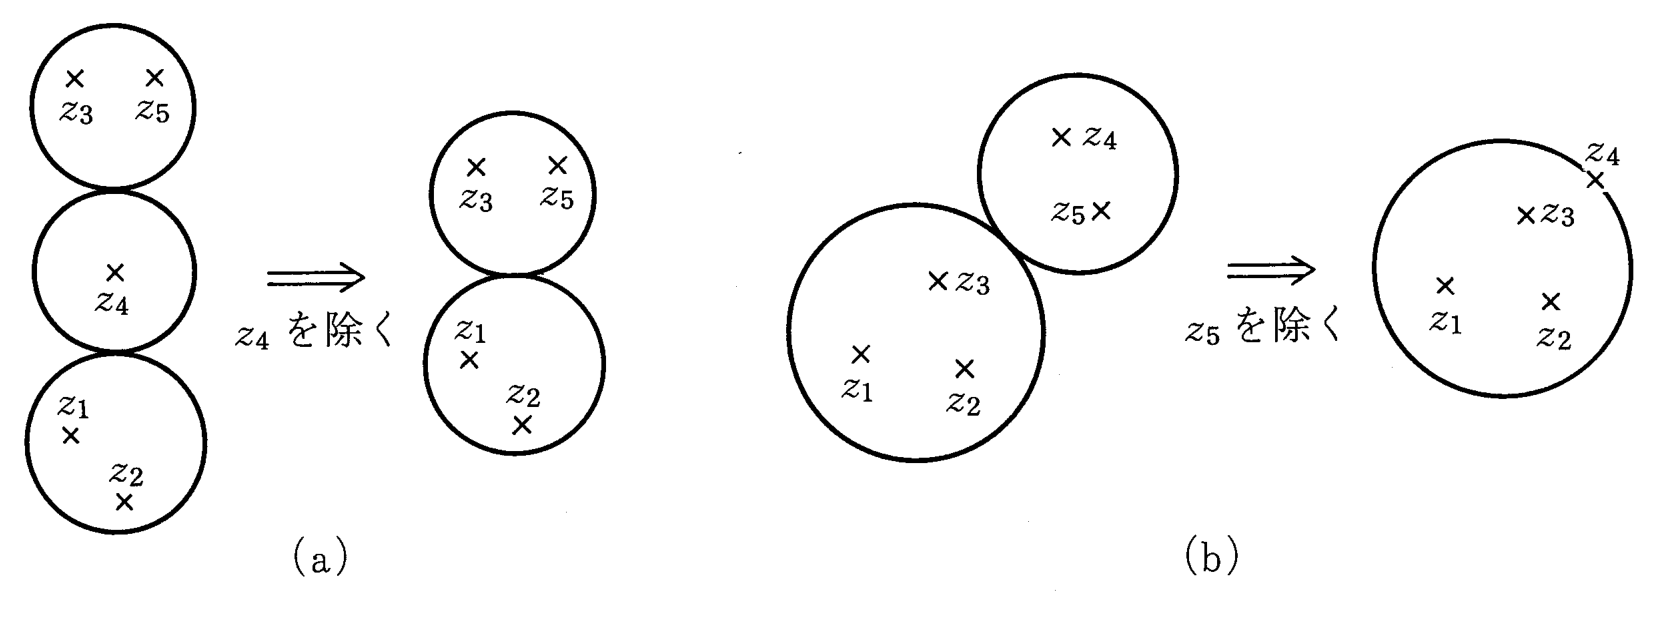
\includegraphics[width=0.86\textwidth]{figures/fig6.8.png}
  \figtitle{6.8}{除去变得不稳定的成分（原书 p.270）}
\end{figure}
\begin{remark}{6.60}
  $\mathrm{fg}:CM_{g,k}(M,J_M;\beta)\to CM_{g,k}$ 的定义也与 $\mathrm{forget}$ 的定义同样。即，忘记映射之后，把变得不稳定的成分缩掉。
\end{remark}
% [Tutor Note: $\mathrm{forget}_h$ 与 $\mathrm{fg}$ 的要点都在“缩掉不稳定成分”这一步：先忘掉带名点，再把特殊点不足 3 个的 $\mathbb P^1$ 成分缩成一点，并相应地合并或新增带名点。这是稳定曲线模空间之间的标准忘却映射。]

% [原文 p.271]
继续定理 6.59 的证明。定义 $h_0:\{1,2,3,4\}\to\{1,2,\dots,k+4\}$ 为 $h_0(1)=1$、$h_0(2)=2$、$h_0(3)=3$、$h_0(4)=k+4$。此时把 $\mathrm{forget}_{h_0}$ 简记为 $\mathrm{forget}$。与定理 6.51 的证明中同样，把图 6.5 的 (1)、(2) 对应的 $CM_{0,4}$ 的点记为 $a,b$。考虑 $\mathrm{forget}^{-1}(a)$，它按第 4 号到第 $k+3$ 号的 $k$ 个带名点位于两个不可约成分 $\Sigma_1$ 与 $\Sigma_2$ 的哪一侧，而分成许多成分。令 $J_1+J_2=\{4,\dots,k+3\}$。对 $i\in J_1$ 的 $i$，第 $i$ 号带名点乘在 $\Sigma_1$ 上；对 $i\in J_2$ 的 $i$，第 $i$ 号带名点乘在 $\Sigma_2$ 上；$\mathrm{forget}^{-1}(a)$ 中这样的元全体，记作 $\mathrm{forget}^{-1}(a)_{J_1,J_2}$。$\mathrm{forget}^{-1}(b)_{J_1,J_2}$ 也类似定义。

令
\begin{equation}
  \mathrm{fg}^{-1}(\mathrm{forget}^{-1}(a)_{J_1,J_2})=M_{0,k+1}(M,J_M;\beta)_{a;J_1,J_2} \tag{6.16}
\end{equation}
这里 $\mathrm{fg}:M_{0,k+1}(M,J_M;\beta)\to M_{0,k+1}$。$M_{0,k+1}(M,J_M;\beta)_{b;J_1,J_2}$ 由在 (6.16) 中把 $a$ 换成 $b$ 来定义。

\begin{lemma}{6.61}
  $\mathrm{m}_{2+\#J_2}^{A,fm}\left(\mathrm{m}_{2+\#J_1}^{A,fm}(P_1,P_2,P_{J_1}),P_3,P_{J_2}\right)$ 与由 $M_{0,k+1}(M,J_M;\beta)_{a;J_1,J_2}$ 给出的对应
  \[
    \left(\textstyle\prod P_i\times_{ev_1,\dots,ev_k}M_{0,k+1}(M,J_M;\beta)_{a;J_1,J_2},ev_{k+1}\right)
  \]
  一致。$\mathrm{m}_{2+\#J_1}^{A,fm}\left(P_1,P_{J_1},\mathrm{m}_{2+\#J_2}^{A,fm}(P_2,P_3,P_{J_2})\right)$ 与由 $M_{0,m+1}(M,J_M;\beta)_{b;J_1,J_2}$ 给出的对应一致。
\end{lemma}

引理 6.61 的证明与引理 6.53 的证明相同。

用引理 6.61 代替引理 6.53，作与定理 6.30 的证明同样的讨论，就得到定理 6.59。

映射 $\mathrm{m}_k^A$ 们包含亏格 0 的 Gromov–Witten 不变量的全部信息。这是下一定理 6.63 的推论。

单连通且连通的紧致 1 维单纯复体称为\textbf{树}（tree）。对亏格 0 的稳定曲线 $\Sigma$，$\Gamma_\Sigma$ 是树。

\begin{definition}{6.62}
  树 $\Gamma$ 中没有出边为 2 条的顶点，出边只有 1 条的顶点数恰为 $k+1$。对出边只有 1 条的顶点，预先确定编号 $1,\dots,k+1$。以上的树全体（与顶点上编号的组）记作 $\mathfrak{T}_{k+1}$。对 $\Gamma\in\mathfrak{T}_{k+1}$，把使 $\Gamma_\Sigma=\Gamma$ 的稳定曲线 $\Sigma$ 全体记作 $CM(\Gamma)$。
\end{definition}

% [原文 p.272]
\begin{theorem}{6.63}
  （Knudsen [202]，Keel [197]）同调群 $H_*(CM_{0,k+1};\Q)$ 由 $CM(\Gamma)$ 的基本同调类们生成。
\end{theorem}

说明如何由定理 6.63 看出映射 $\mathrm{m}_k^A$ 们包含亏格 0 的 Gromov–Witten 不变量的全部信息。设 $\Gamma\in\mathfrak{T}_{k+1}$，则 $H^*(M;\Lambda_{nov})$ 的元素之间 $\mathrm{m}_k$ 们如何合成就确定了。与其用一般语言说明，不如看例子。图 6.9 的 (a)、(b)、(c) 分别是
\[
  \mathrm{m}_2(x_1,\mathrm{m}_2(x_2,x_3)),\qquad
  \mathrm{m}_3(x_1,x_2,x_3),
\]
\[
  \mathrm{m}_4\left(\mathrm{m}_2(\mathrm{m}_3(x_1,x_2,x_3),x_4),\mathrm{m}_2(x_5,x_6),x_7,x_8\right).
\]
把这个合成记作 $\mathrm{m}_\Gamma^{A,fm}:H^*(M;\Lambda_{nov})^{\otimes k}\to H^*(M;\Lambda_{nov})$。它与 (6.15) 同样分解为 $\mathrm{m}_{\Gamma,\beta}^{A,fm}$。与定理 6.59 的证明同样，可得下述引理。

\begin{figure}[htbp]
  \centering
  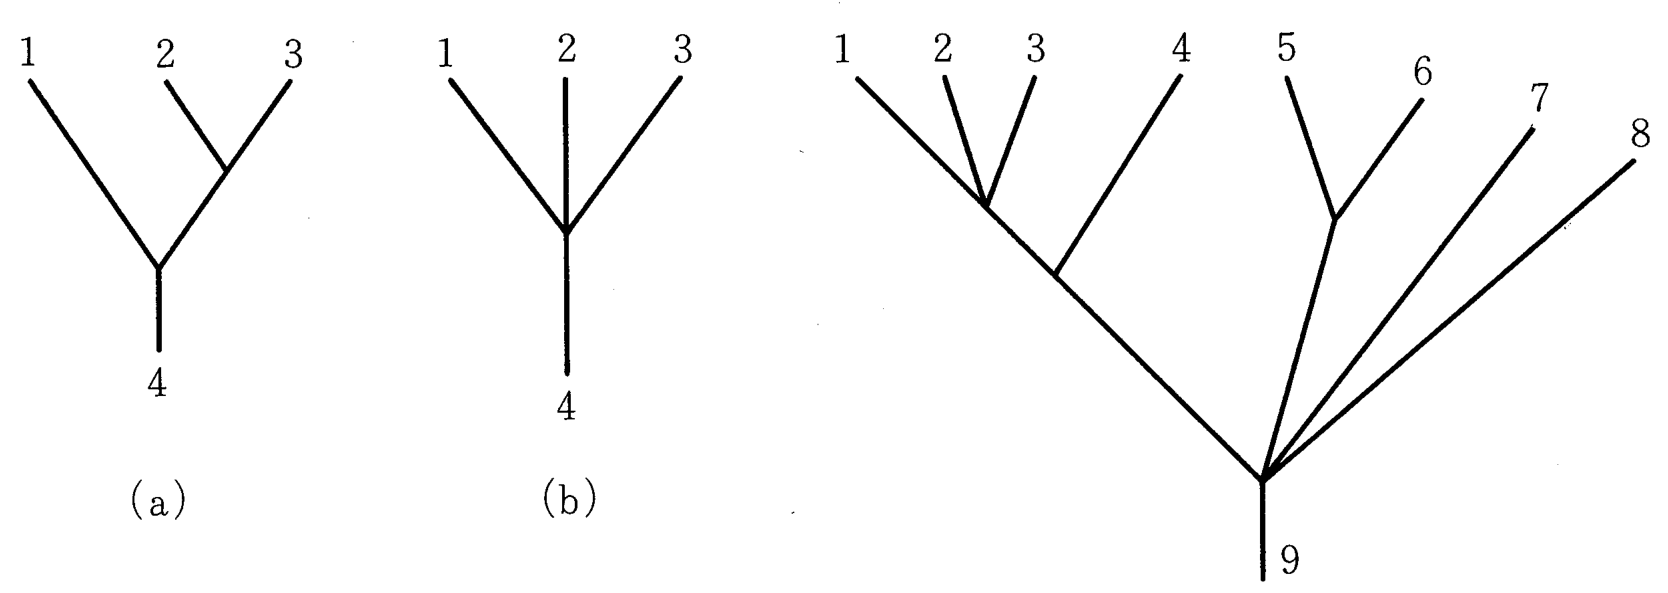
\includegraphics[width=0.86\textwidth]{figures/fig6.9.png}
  \figtitle{6.9}{$\Gamma$ 与 $\mathrm{m}$ 的对应（原书 p.272）}
\end{figure}

\begin{lemma}{6.64}
  \[
    \mathrm{m}_{\Gamma,\beta}^A(P_1,\dots,P_k)=\sum_\beta\left(\textstyle\prod P_i\times_{ev_1,\dots,ev_k}CM_\Gamma(M,J_M;\beta),ev_{k+1}\right)T^{\beta\cap\omega_M}\otimes u^{c^1(M)\cap\beta}.
  \]
\end{lemma}

引理 6.64 与定理 6.63 表明，亏格 0 的 Gromov–Witten 不变量全部可表为 $\mathrm{m}_k$ 们的合成的线性组合。

同样，$\mathrm{m}_k$ 们的合成应满足的关系式也由定理 6.59 穷尽。这是下一定理 6.65 的推论。设 $h:\{1,\dots,m+1\}\to\{1,\dots,k+1\}$ 为

% [原文 p.273]
单射。定义 $\mathfrak{sh}_h:\mathfrak{T}_{k+1}\to\mathfrak{T}_{m+1}$。设 $\Gamma\in\mathfrak{T}_{m+1}$。把 $\Gamma$ 中编号为 $h(1),\dots,h(m+1)$ 的顶点以及从它们出发的外线全部去掉。于是某些顶点只剩 1 条或 2 条边。除编号为 $h(1),\dots,h(k+1)$ 的顶点以外，把它们取掉。取掉出边为 1 条的顶点时，从其出发的边也取掉。取掉出边为 2 条的顶点时，把出边接成 1 条边。反复此操作，就得到 $\mathfrak{T}_{m+1}$ 的元素。
% [Tutor Note: 原书 p.273 定义 $\mathfrak{sh}_h$ 处 $k$ 与 $m$ 的下标有互换：映射写作 $\mathfrak{T}_{k+1}\to\mathfrak{T}_{m+1}$，却又设 $\Gamma\in\mathfrak{T}_{m+1}$，末句又得到 $m+1$ 条外线。按 (6.17) 的用法，应读作“从 $(k+1)$ 条外线的树 $\Gamma$ 出发，去掉编号 $h(1),\dots,h(m+1)$ 的外线，缩掉次数 1、2 的顶点，得到 $(m+1)$ 条外线的树”。]

定义 $h_0:\{1,2,3,4\}\to\{1,\dots,k+1\}$ 为 $h_0(1)=1$、$h_0(2)=2$、$h_0(3)=3$、$h_0(4)=k+1$。把 $\mathfrak{sh}_{h_0}$ 简记为 $\mathfrak{sh}$。由定义，
\begin{equation}
  \mathrm{fg}^{-1}(CM_{0,4}(\Gamma))=\sum_{\Gamma,\ \mathfrak{sh}(\Gamma)=\Gamma}CM_{0,k+1}(\Gamma) \tag{6.17}
\end{equation}
成立。（(6.17) 可推广为 $\mathrm{forget}_h:CM_{0,k+1}(\Gamma)\to CM_{0,m+1}(\Gamma)$ 与 $\mathfrak{sh}_h$ 之间的类似关系。）设 $\Gamma_1,\Gamma_2\in\mathfrak{T}_4$ 为图 6.5 的 (a)、(b) 的图。由 (6.17) 得
% [Tutor Note: (6.17) 的求和式中，作为求和变量的 $\Gamma$ 与右边固定的 $\Gamma$ 用了同一个字母，容易误读。应读作：对满足 $\mathfrak{sh}(\Gamma')=\Gamma$ 的所有 $\Gamma'$ 求和。]

\begin{equation}
  \sum_{\Gamma\in\mathfrak{T}_{m+1},\ \mathfrak{sh}(\Gamma)=\Gamma_1}[CM_{0,k+1}(\Gamma)]=\sum_{\Gamma\in\mathfrak{T}_{m+1},\ \mathfrak{sh}(\Gamma)=\Gamma_2}[CM_{0,k+1}(\Gamma)] \tag{6.18}
\end{equation}
这一 $H_*(CM_{0,k+1};\Q)$ 中的等式。

\begin{theorem}{6.65}
  （Knudsen [202]，Keel [197]）式 (6.18) 是 $[CM_{0,m+1}(\Gamma)]$ 所满足的关系式的全部。即 $H_*(CM_{0,k+1};\Q)$ 是由 $[CM_{0,m+1}(\Gamma)]$ 生成、以 (6.18) 为基本关系式的向量空间。
\end{theorem}

为了说明定理 6.59 的关系式的背景，下面叙述 operad。

\begin{definition}{6.66}
  对每个自然数 $k$ 有空间 $\mathfrak{P}(k)$，其上有 $k$ 次置换群 $\mathfrak{S}_k$ 作用，并且存在连续映射
  \[
    \mathrm{Comp}:\mathfrak{P}(k)\times\prod_{i=1}^k\mathfrak{P}(m_i)\longrightarrow\mathfrak{P}(m_1+\dots+m_k),
  \]
  满足下述公理时，这些称为 \textbf{operad}（操作子）（或拓扑空间的 operad）。
  \begin{enumerate}[label=（\arabic*）]
    \item 对 $\sigma\in\mathfrak{S}_k$、$f\in\mathfrak{P}(k)$、$g_i\in\mathfrak{P}(m_i)$，下式成立：
% [原文 p.274]
    \[
      \mathrm{Comp}(\sigma f;g_{\sigma1},\dots,g_{\sigma k})=\mathrm{Comp}(f;g_1,\dots,g_k).
    \]
    \item 对 $f\in\mathfrak{P}(k)$、$g_i\in\mathfrak{P}(m_i)$、$h_{i,j}\in\mathfrak{P}(m_{i,j})$，下式成立：
\[
  \resizebox{0.97\linewidth}{!}{$\displaystyle \mathrm{Comp}\left(f;\mathrm{Comp}(g_1;h_{1,1},\dots,h_{1,m_1}),\dots,\mathrm{Comp}(g_k;h_{k,1},\dots,h_{k,m_k})\right) =\mathrm{Comp}\left(\mathrm{Comp}(f;g_1,\dots,g_k);h_{1,1},\dots,h_{k,m_k}\right). $}
\]
  \end{enumerate}
\end{definition}

当 $\mathfrak{P}(k)$ 是向量空间、$\mathrm{Comp}$ 是从张量积出发的线性映射时，若也满足上述定义的 (1)、(2)，则称为 operad（或向量空间的 operad）。

下面定义的 operad 上的模，大体上可以认为就是有以 $\mathfrak{P}(k)$ 为参数、以 $H^{\otimes k}\to H$ 为型的积的结构。

\begin{definition}{6.67}
  设 $H$ 为分次向量空间。若给定映射 $\mathrm{m}:\mathfrak{P}(k)\times H^{\otimes k}\to H$，固定 $\mathfrak{P}(k)$ 的元就导出同态 $H^{\otimes k}\to H$，并且满足下列性质，则称 $H$ 是 operad $(\mathfrak{P}(k),\mathrm{Comp})$ 上的\textbf{模}。
  \begin{enumerate}[label=（\arabic*）]
    \item 对 $\sigma\in\mathfrak{S}_k$、$f\in\mathfrak{P}(k)$、$x_i\in H$，下式成立：
    \[
      \mathrm{m}(\sigma f;x_{\sigma1},\dots,x_{\sigma k})=\pm\mathrm{m}(f;x_1,\dots,x_k).
    \]
    这里 $\pm$ 是把 $x_1,\dots,x_k$ 换成 $x_{\sigma1},\dots,x_{\sigma k}$ 时出现的符号。
    \item 对 $f\in\mathfrak{P}(k)$、$g_i\in\mathfrak{P}(m_i)$、$x_{i,j}\in H$，下式成立：
\[
  \resizebox{0.97\linewidth}{!}{$\displaystyle \mathrm{m}\left(f;\mathrm{m}(g_1;x_{1,1},\dots,x_{1,m_1}),\dots,\mathrm{m}(g_k;x_{k,1},\dots,x_{k,m_k})\right) =\mathrm{m}\left(\mathrm{Comp}(f;g_1,\dots,g_k);x_{1,1},\dots,x_{k,m_k}\right). $}
\]
  \end{enumerate}
\end{definition}

\begin{example}{6.68}
  令 $\mathfrak{P}(k)=M_{0,k+1}$，$\mathfrak{S}_k$ 的作用为调换 $1,\dots,k$ 号带名点的顺序。如下定义 $\mathrm{Comp}$。设 $(\Sigma,\vec z)\in M_{0,k+1}$、$(\Sigma_i,\vec z^i)\in M_{0,m_i+1}$（记 $\vec z=(z_1,\dots,z_k)$、$\vec z^i=(z^i_1,\dots,z^i_{m_i})$）。$\mathrm{Comp}((\Sigma,\vec z);(\Sigma_1,\vec z^1),\dots,(\Sigma_k,\vec z^k))$ 定义为这样的半稳定曲线：$\Sigma,\Sigma_i$ 为非奇异不可约成分，$z_i\in\Sigma=z^i_{m_i+1}\in\Sigma_i$ 为奇点，$z^1_1,\dots,z^1_{m_1},\dots,z^k_1,\dots,z^k_{m_k}$ 为带名点。换句话说，它是把 $\Sigma_i$ 与 $\Sigma$ 在 $z_i$ 与 $z^i_{m_i+1}$ 处粘合起来的半稳定曲线（图 6.10）。容易看出 $\mathrm{Comp}$ 可扩充到 $CM_{0,k+1}\times\prod CM_{0,m_i+1}$，并确定一个 operad。
\end{example}

\begin{example}{6.69}
  令 $\mathfrak{P}(k)=H_*(CM_{0,k+1})$，$\mathrm{Comp}$ 为例 6.68 的映射在同调上诱导的映射，则得到向量空间的 operad。
\end{example}

% [原文 p.275]
\begin{figure}[htbp]
  \centering
  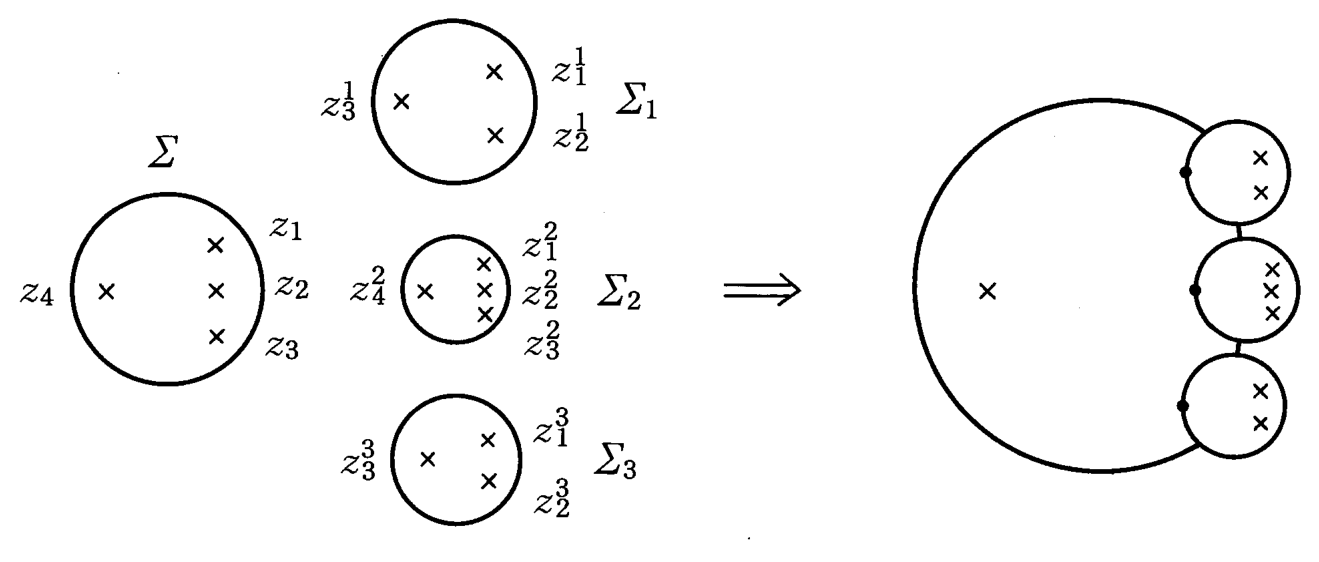
\includegraphics[width=0.80\textwidth]{figures/fig6.10.png}
  \figtitle{6.10}{operad 与 $M_{0,n}$（原书 p.275）}
\end{figure}

\begin{example}{6.70}
  设 $(M,J_M,\omega)$ 为辛流形，$H$ 为 $M$ 的上同调群。设 $y\in H_*(CM_{0,k+1})$，$x_1,\dots,x_{k+1}\in H$。设 $y$ 的 Poincaré 对偶为 $y^*$。用 Gromov–Witten 不变量与斜积定义
  \[
    \mathrm{m}(y;x_1,\dots,x_k)=\mathrm{GW}_{0,k+1}(M,J_M,\omega)\backslash(y^*\times x_1\times\dots\times x_k)\in H^*(M).
  \]
  容易看出 $\mathrm{m}$ 确定例 6.69 的 operad 上的模结构。
\end{example}

下一定理 6.72 是先前提过的事情，即（亏格 0 的）Gromov–Witten 不变量的基本关系式就是定理 6.59 的 Comm$_\infty$ 关系式，这一说法的另一种表述。在它之前先定义 Comm$_\infty$ 代数。

\begin{definition}{6.71}
  向量空间 $H$ 上的 \textbf{Comm$_\infty$ 代数}结构，是指线性映射族 $\mathrm{m}_k:H^{\otimes k}\to H$，满足
  \[
    \mathrm{m}(\dots,x_i,x_{i+1},\dots)=(-1)^{\deg x_i\deg x_{i+1}}\mathrm{m}(\dots,x_{i+1},x_i,\dots)
  \]
  以及定理 6.59 结论中的式子成立。
\end{definition}

\begin{theorem}{6.72}
  （Ginzburg–Kapranov [142]）Comm$_\infty$ 代数结构与例 6.69 的 operad 上的模结构一一对应。
\end{theorem}

证明只要好好考虑定理 6.63 与 6.65，就显然。

operad 的概念由 May [249] 提出。（在此前后，Boardman–Vogt [45]、Stasheff [347] 等人研究了类似概念\footnote{更早地，在 Kolmogorov–Arnold 关于 Hilbert 第 13 问题（$n$ 个变量的任意函数能否表示为由更少变量的函数复合而成）的研究 [213], [8] 中，可以看到类似想法的萌芽。}。）关于这些，[3] 是优秀的教科书。

% CHUNK ch06a2 DONE

